%
%  $Description: Survey on Orchestration$
%

\documentclass[10pt,twocolumn]{article}
\usepackage{times,mathptmx,fullpage}
% Allows you to put literal text into your document without having LaTeX try to interpret it.
\usepackage{verbatim}
% Sorts citations numerically and "combines" adjacent ones
\usepackage{cite}
% Allows you to individually label subfigures in a multi-part figure
\usepackage{subfigure}
% Allows the definition of macros that are smart about adding space
% after text in a macro
\usepackage{xspace}
% To use external images
\usepackage{graphicx}

% Redefine the percentage of the page that can be used for floats (figures, tables, etc.)
\renewcommand\floatpagefraction{.9}
\renewcommand\dblfloatpagefraction{.9}
\renewcommand\topfraction{.9}
\renewcommand\dbltopfraction{.9}
\renewcommand\bottomfraction{.9}
\renewcommand\textfraction{.1}
\setcounter{totalnumber}{10}
\setcounter{topnumber}{10}
\setcounter{dbltopnumber}{10}
\setcounter{bottomnumber}{10}

% Set values for float separation from text
\setlength{\floatsep}{1.5ex plus1.0ex minus 0.2ex}
\setlength{\dblfloatsep}{1.5ex plus1.0ex minus 0.2ex}
\setlength{\textfloatsep}{1.5ex plus1.0ex minus 0.2ex}
\setlength{\dbltextfloatsep}{1.5ex plus1.0ex minus 0.2ex}
\setlength{\abovecaptionskip}{0.5ex}
\setlength{\belowcaptionskip}{0.5ex}

% Don't allow widows or clubs - single lines at the start/end of a column
\widowpenalty=10000
\clubpenalty=10000

\newcommand{\latex}{\LaTeX\xspace}
\pagestyle{plain}

%-------------------------------------------------------------------------
\begin{document}

\title{A Survey on Virtual Machine and Container Orchestration}

\author{
Aneesh Neelam \\
\textit{Univ. of California, Santa Cruz} \\
\textit{aneelam@ucsc.edu}
}

\maketitle
\thispagestyle{empty}

\begin{abstract}

  Data center administrators and site-reliability engineers create virtual machines or containers to run their applications, with desired redundancy requirements and automated coordination between the replicas.
  This is called the orchestration of the various computing, storage and network resources of the data center.
  To automate the orchestration process, different tools have been developed in the past couple of decades.
  Each tool was designed differently, with different intents and priorities but they also have a lot in common.
  This survey is on the various orchestration tools available to data center administrators, site reliability engineers and software engineers;
  and aims to be a comprehensive guide that helps data center administrators in choosing the cloud platform and the orchestration tool.

\end{abstract}

%-------------------------------------------------------------------------
\section{Introduction}

With the advent and proliferation of virtualization, computing as a service has taken off.
Now there are multiple cloud service providers such as Google Cloud, Amazon Web Service, Microsoft Azure etc.
The operators of these cloud services typically have their own data centers, each consisting of thousands of physical machines connected via a high speed and very low latency network such as Infiniband (IB) ~\cite{intro_infiniband}.
Data center operators use various tools to automate the process of management, provisioning and scaling the resources for their customers.

Orchestration tools have been developed to ease the automation of operating a data center.
Tools such as VMware vCenter Orchestrator and Microsoft System Center Orchestrator, and OpenStack's Heat have been used to manage VMware vSphere, Microsoft Hyper-V or Linux kernel virtual machines.
Container Orchestration tools such as Docker Swarm, Kubernetes, Mesos have been developed to manage containers on mostly Linux machines, but also increasingly on Windows machines as well ~\cite{docker_swarm, kubernetes, mesos}.

%-------------------------------------------------------------------------
\section{Background}

The increasing proliferation and popularity of virtualization technology was necessary for the data center, and cloud service providers to thrive.
Consequently, cloud computing has made the concept of computing as a utility possible ~\cite{berkeley_cloud}.
Virtualization, in this context, is the task of creating virtual hardware and running actual operating systems and applictions on top of them.
Each of these virtual machines are isolated and independent from one another, and are managed by a hypervisor that is running on the physical hardware or on the host operating system ~\cite{xen}.

\begin{figure*}
\centering
  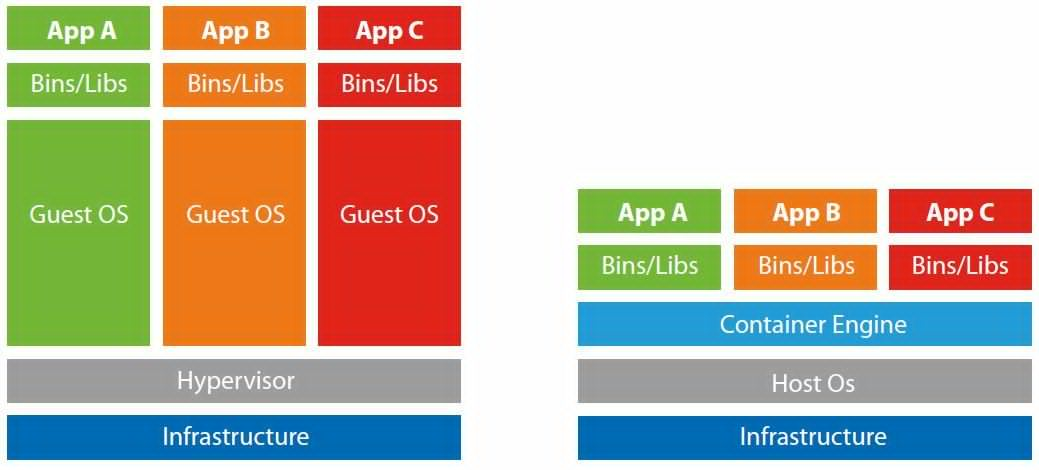
\includegraphics[width=\textwidth]{container-vs-vm.jpg}
    \caption{Differences between Virtual Machines and Containers~\cite{intro_containerisation}
      \label{overflow}}
\end{figure*}

%-------------------------------------------------------------------------
\section{General Comparison}



\subsection{Virtual Machine Orchestration}



\subsection{Container Orchestration}



%-------------------------------------------------------------------------
\section{Evaluations}



\subsection{Performance}



\subsection{Ease of Use}



\subsection{Protocols used}



\subsection{Use Cases}



\subsection{Caveats}




%-------------------------------------------------------------------------
\section{Future of Orchestration}



\subsection{Use of Virtual Machines}



\subsection{Innovation in Tools}



%-------------------------------------------------------------------------
\section{Conclusion}



%-------------------------------------------------------------------------
\bibliographystyle{latex8}
\bibliography{orchestration}

\end{document}
